% CQG submission version derived from the audited journal-agnostic preprint.
\documentclass{iopjournal}
\usepackage{amsmath,amssymb,mathtools,mathrsfs,microtype,booktabs,tabularx,array,float}
\newcolumntype{Y}{>{\raggedright\arraybackslash}X}
\setlength{\emergencystretch}{2em}
\hypersetup{pdftitle={Boundary-State Sufficiency in Gowdy Cosmology},pdfauthor={Ronald Bibb}}

\begin{document}
\articletype{Paper}
\title{Boundary-State Sufficiency in Gowdy Cosmology: Smooth Closure Does Not Extend Through Spikes}
\author{Ronald Bibb\orcid{0009-0004-1153-2464}}
\affil{Independent Researcher, Lilburn, GA 30047, USA}
\email{ronbibb@gmail.com}
\par\noindent\keywords{cosmological singularities, Gowdy spacetimes, Fuchsian asymptotics, numerical relativity, spike solutions}\par

\begin{abstract}
Singular asymptotic data can parameterize important classes of cosmological solutions, but this does not ensure that a reduced state inferred from finite-time Cauchy evolution retains every datum needed to reconstruct a chosen geometric state. We test that sufficiency directly: boundary data are extracted on a finite-depth window, the intervening history is discarded, a second branch is initialized from the declared boundary object, and invariant observables are compared after the declared time-parity map. In smooth polarized Gowdy $T^3$ Einstein--scalar data, predictive field reconstruction and exact multimode Bessel benchmarks converge at second order. Four field functions recover normalized shape, while full marked geometry additionally requires the additive metric modulus. The same diagnostic fails locally in nonlinear vacuum unpolarized data: near two resolved spike candidates the reconstruction distance is $(0.8201,0.8169,0.8222)$ for $N=(1024,2048,4096)$. Exact true-spike controls identify representation loss rather than truncation error: ordinary four-function velocity-dominated data give a known-answer distance $0.5715$, whereas an enriched centered-spike state reduces it to $2.38\times10^{-4}$. Thus smooth closure does not license exceptional closure. The result is observable- and model-relative; it establishes neither generic almost-everywhere sufficiency nor a physical continuation law through the singularity.
\end{abstract}

\section{Introduction}
Fuchsian methods show that prescribed singular data generate important classes of cosmological solutions [1--6], while geometric singular initial-value and scattering-map frameworks clarify which data may be assigned at a singular hypersurface [7--9]. A different question arises when the data are not prescribed as truth but inferred from an ordinary Cauchy evolution: has the proposed compression retained enough information to reconstruct the geometric observables of interest?

We make that question falsifiable with an extraction--reconstruction diagnostic,
\[
\mathscr C_-\xrightarrow{\mathcal E}\mathscr B_{\rm adm}
\xrightarrow{\mathcal R}\mathscr C_+
\xrightarrow{\mathcal O,\mathcal T}D,
\]
where $\mathcal E$ extracts constrained asymptotic data, $\mathcal R$ initializes a separate branch, $\mathcal O$ constructs geometric observables, and $\mathcal T$ applies the declared reversal of the future normal. Formal time reversibility is not enough: endpoint fields, constraint data, or a global metric anchor can otherwise pass silently between the two branches. The diagnostic therefore separates predictive extraction from endpoint copying and distinguishes normalized shape from marked geometry.

The result has three linked parts. First, smooth polarized field data close predictively under refinement. Second, those four functions determine normalized shape but not full marked geometry; the additive metric modulus is load bearing. Third, ordinary four-function velocity-dominated (VTD) data fail by a resolution-stable margin near nonlinear unpolarized spike candidates. On exact spike controls, an enriched family-specific state repairs precisely the information lost by the ordinary VTD compression. The last result is the central one: a representation validated in a smooth sector need not remain sufficient on an exceptional set.

The exceptional analytical status of Gowdy spikes is established [11--13,18--20]. Our contribution is operational and quantitative: a declared invariant score measures reconstruction loss, refinement distinguishes that loss from discretization error, and exact controls identify an enrichment that restores the tested family. We do not claim a new spike solution, a generic almost-everywhere theorem, or a physical map through the singularity.

Figure~\ref{fig:architecture} summarizes the inference. Section 2 defines only the state and score needed to read the results. Sections 3--5 present smooth closure, the global-modulus requirement, and spike-localized failure. The appendices record mathematical conventions and compact derivations; the accompanying supplement gives the complete numerical protocol, control definitions, tolerances, and extended results.

\begin{figure}[H]
\centering
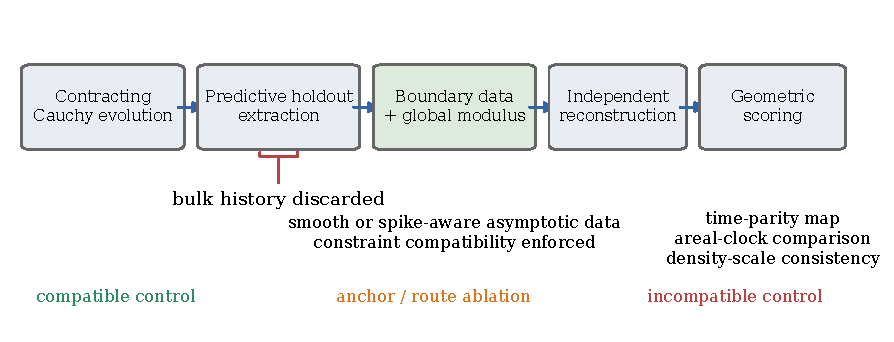
\includegraphics[width=0.97\textwidth]{figures/output/figure_1_method_architecture.pdf}
\caption{The extraction--reconstruction test. The reconstruction branch receives only the declared boundary object; agreement is judged with geometric observables after the stated parity map.}
\label{fig:architecture}
\end{figure}

\section{Boundary state and sufficiency test}
\subsection{Smooth polarized state}
For polarized Gowdy $T^3$ Einstein--scalar data in areal time $\tau$, the field asymptotics are
\[
P=v_P\tau+P_\infty+r_P,\qquad
\phi=v_\phi\tau+\phi_\infty+r_\phi .
\]
The four shape functions form
\[
\mathfrak B_{\rm shape}=(v_P,v_\phi,P_\infty,\phi_\infty).
\]
Writing $q=v_P^2+v_\phi^2$, the constrained metric field satisfies
\[
\lambda=q\tau+\lambda_\infty+r_\lambda,qquad
\partial_\theta\lambda_\infty=2(v_P\partial_\theta P_\infty+v_\phi\partial_\theta\phi_\infty).
\]
The momentum constraint fixes only the nonconstant part of $\lambda_\infty$. With the $T^3$ marking and periods fixed, full data therefore require
\[
\mathfrak B_{\rm full}=(v_P,v_\phi,P_\infty,\phi_\infty,c_\lambda;L_\theta,L_x,L_y),
\qquad c_\lambda=\lambda_\infty(0).
\]
This is a claim relative to the fixed marking: if the marking and its periods are relaxed, the corresponding scale direction may instead be quotiented. Appendix A gives the metric conventions, constraints, admissibility condition, and normalization details.

Extraction is predictive in the field sector. For $f\in\{P,\phi\}$, the principal estimator uses only the holdout interval $[\tau_f-2\Delta,\tau_f-\Delta]$,
\[
v_f^{\rm hold}=\frac{f(\tau_f-\Delta)-f(\tau_f-2\Delta)}{\Delta},\qquad
f_\infty^{\rm hold}=f(\tau_f-\Delta)-v_f^{\rm hold}(\tau_f-\Delta),
\]
and predicts the discarded endpoint. The production metric route retains a finite-depth collapse-side anchor and is therefore not a source-independent recovery of the modulus. The exact benchmark removes that dependence by supplying the limiting five-part object analytically. The endpoint baseline and the precise independence hierarchy are documented in Supplement Secs. S2--S4.

\subsection{Unpolarized test state}
For vacuum unpolarized Gowdy data, the ordinary tested VTD state is
\[
\mathfrak B_{\rm VTD}=(v,P_\infty,Q_\infty,\pi_Q),
\qquad \pi_Q=e^{2P}Q_{,\tau},
\]
with $P\sim v\tau+P_\infty$. This representation is not assumed sufficient at a spike. Exact true- and false-spike families [11,18] test both the nonlinear evolution and the information retained by the compression. A family-specific enriched control state additionally retains $(w,Q_0,Q_2,x_0)$. Its success establishes repair on that exact family, not identification of the production feature with a Lim solution.

\subsection{Observable-relative criterion}
Future-normal reversal maps $(g_{ij},K_{ij},\phi,n\phi)$ to $(g_{ij},-K_{ij},\phi,-n\phi)$. We score the even normalized observables $(\Omega,\Sigma^2,s_P)$ together with the parity-adjusted dimensionless clock observable $\Theta\lambda_A$, where $\lambda_A=e^{-\tau/2}$. On each comparison surface,
\[
D(\tau)=\sup_\theta\left\|\mathfrak O_{s,-}(\tau,\theta)-\mathcal T\mathfrak O_{s,+}(\tau,\theta)\right\|_2 .
\]
The density scale $\lambda_\rho=\rho^{-1/2}$ supplies an independent clock-consistency check. Passing means convergence and satisfaction of the frozen criterion for the declared family, marking, reconstruction, observables, clocks, parity, norm, and tolerances. It does not prove injectivity on the full geometric state space. Supplement Secs. S3--S4 give the complete score, sampled surfaces, gates, and control matrix.

\section{Smooth predictive closure}
We first ask whether finite-window data reconstruct the smooth polarized field sector without reading the endpoint fields. The risk is endpoint copying or finite-depth contamination masquerading as asymptotic sufficiency. The criterion is predictive holdout accuracy together with refinement and extraction-depth consistency.

The holdout reconstruction converges at second order in both the production calculation and exact multimode Bessel tests. In the latter, the limiting coefficients are known analytically from
\[
f_k=[A_kJ_0(ke^{-\tau})+B_kY_0(ke^{-\tau})]T_k(\theta),
\quad v_k=-\frac{2B_k}{\pi},
\]
so extraction error and forward-reconstruction error can be separated. Figure~\ref{fig:smooth} shows the representative convergence result; Supplement Secs. S4--S6 give the resolution sets, score definitions, acceptance criteria, control outcomes, and extended error-budget evidence. The complete machine-readable field, clock, and constraint histories are retained in the repository.

\begin{figure}[H]
\centering
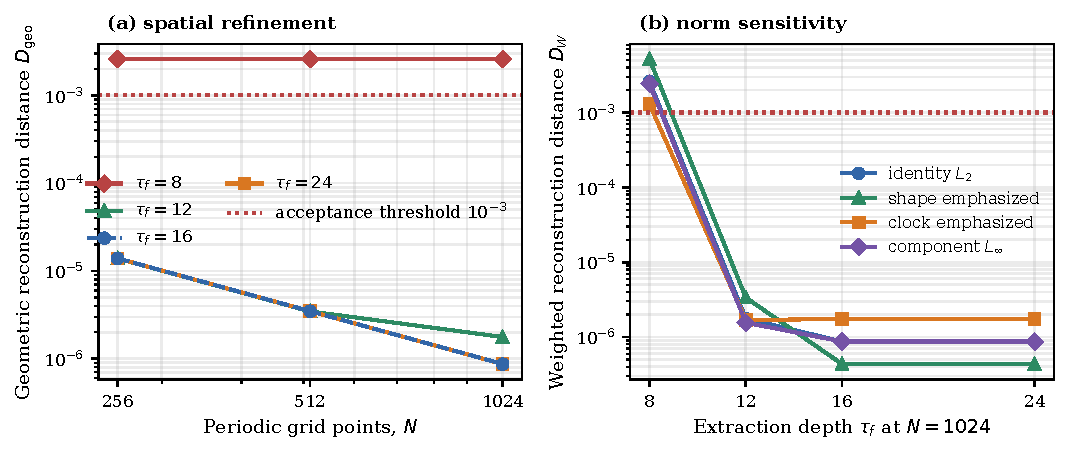
\includegraphics[width=0.92\textwidth]{figures/output/figure_2_production_convergence.pdf}
\caption{Representative predictive smooth-sector convergence. The resolution sets, frozen acceptance criteria, and extended error-budget evidence are reported in the supplement; complete machine-readable sequences remain in the repository.}
\label{fig:smooth}
\end{figure}

This result supports observable-relative closure of the smooth field and normalized-shape sector. It is deliberately bounded. At the deepest extraction surfaces the analytic remainder is already below the spatial error, so the calculation is a weak stress test of the asymptotic model. It also does not yet establish recovery of full marked geometry, which carries an independent global metric degree of freedom.

\section{The global modulus separates shape from marked geometry}
We next test whether the four smooth field functions determine absolute geometry. The risk is that agreement of scale-free observables conceals a missing global metric mode. The decisive control is an ablation: reconstruct once with $c_\lambda$ retained and once with it removed while holding the shape data fixed.

The normalized shape score is insensitive to this ablation, but absolute clock and proper-length observables are not. Restoring $c_\lambda$ repairs the full score; omitting it produces a nonconvergent geometric offset. The exact Fuchsian benchmark, in which $c_\lambda$ and the remainders are analytically known, independently validates the forward reconstruction. Figure~\ref{fig:modulus-ablation} displays the separation; estimator convergence, the known-answer remainder test, and the full error budget appear in Supplement Sec. S7.

\begin{figure}[H]
\centering
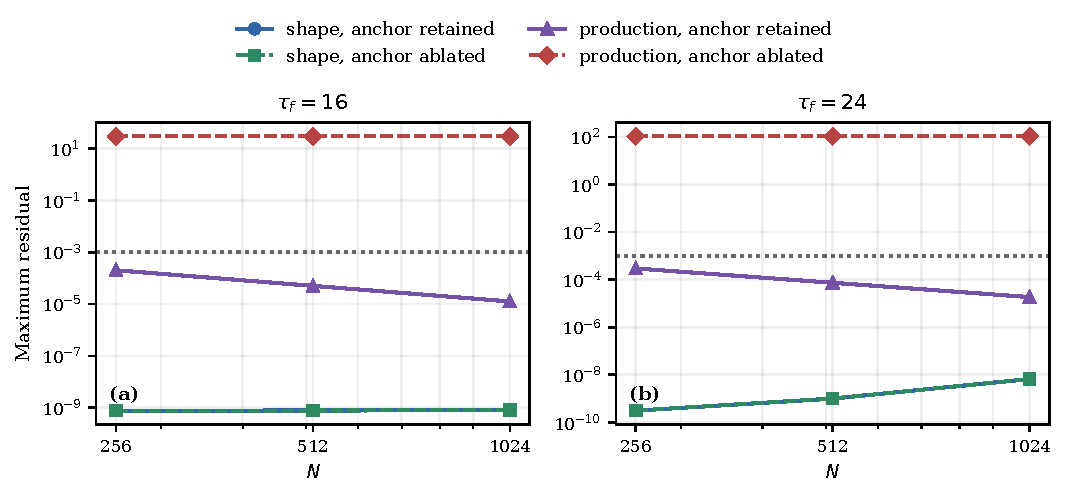
\includegraphics[width=0.94\textwidth]{figures/output/figure_4_global_modulus_ablation.pdf}
\caption{Global-modulus ablation. Four field functions recover normalized shape, whereas full marked geometry requires the additive metric datum $c_\lambda$.}
\label{fig:modulus-ablation}
\end{figure}

The consequence is not the discovery of an unfamiliar Gowdy degree of freedom. It is the demonstrated inferential distinction between two closure claims: four functions suffice for the tested normalized shape, while the five-part constrained object is required for the tested marked geometry.

\section{Spike-localized insufficiency}
The smooth result does not test exceptional unpolarized structure. We therefore apply the same inference to nonlinear vacuum data containing two resolved spike candidates. The question is whether ordinary four-function VTD compression preserves the localized state. The criterion is not a single large residual: failure must remain localized, resolved, and stable under refinement, and exact controls must distinguish representation loss from an incorrect solver or detector.

The localized reconstruction distances are
\[
D_{\rm loc}=(0.8201,0.8169,0.8222)
\quad\hbox{for}\quad N=(1024,2048,4096).
\]
The feature remains resolved while the surrounding reconstruction error decreases, so the discrepancy does not approach a truncation floor. Ordinary VTD data are therefore insufficient in the localized region. Because the fixed ordinary-region mask is contaminated by the wider feature footprint, no almost-everywhere conclusion is drawn.

Exact controls identify what failed. For an exact true spike, compression to ordinary four-function VTD data produces a known-answer center distance of $0.57150$. Retaining the enriched centered-family parameters reduces the maximum distance to $2.3812\times10^{-4}$ at $\tau=2$ and $2.2421\times10^{-5}$ at $\tau=4$. Thus the diagnostic both rejects the ordinary representation and identifies a state that preserves the tested exact family.

\begin{figure}[H]
\centering
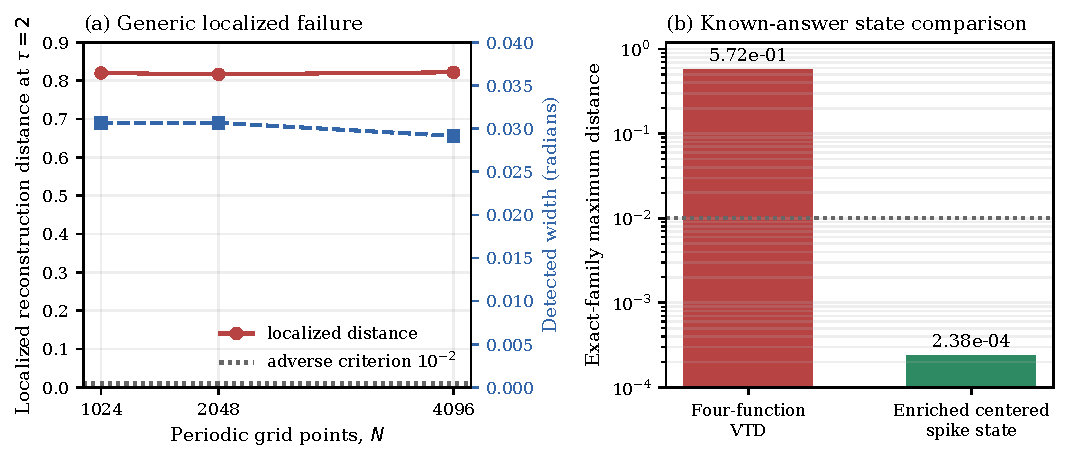
\includegraphics[width=0.96\textwidth]{figures/output/figure_6_unpolarized_spike_extension.pdf}
\caption{Nonlinear extension. The production discrepancy is localized and resolution stable. Exact controls show loss under ordinary VTD compression and repair under the enriched centered-family state.}
\label{fig:spike}
\end{figure}

The controls address three specific alternatives. Analytic differentiation satisfies the amended exact equations to $3.11\times10^{-15}$, while literal printed alternatives fail and serve as negative controls. Integer cyclic shifts give an exact discrete equivariance check; they are not evidence of positional robustness. Separate unseen half-cell shifts converge at approximately second order and remain below $10^{-2}$ on the finest grids. Full residuals, shifted-family sequences, observed orders, detector definitions, and false-spike controls are reported in Supplement Secs. S8--S10.

The production feature is accordingly called a resolved spike candidate, not a member of the exact family. A later dual-scale footprint test localized the exceptional region but did not establish zero-measure decay within its sealed interval; deeper calculations stopped when the narrowing feature failed the resolution criterion. Those outcomes restrict the inference rather than supporting either zero-measure equivalence or a finite-width wall.

\section{Discussion}
The analytical literature treats spikes as exceptional points of ordinary VTD asymptotics [11--13,18]. The present result adds a quantitative reconstruction statement: a finite-time Cauchy history can be compressed into a state that succeeds in a smooth sector yet loses an order-unity amount of declared observable information near a resolved exceptional feature. Exact-family controls then show that the loss belongs to the representation, not merely to the evolution code.

This direction of inference distinguishes the diagnostic from a Fuchsian construction. Fuchsian theory begins with admissible singular data and proves or computes a development. Here the singular data are estimated from a regular solution and then tested for retention of a declared geometric state. The two approaches are complementary: exact Fuchsian data validate the forward leg, while predictive extraction tests whether finite-depth evolution recovers those data without hidden endpoint access.

The calculation also distinguishes boundary-state testing from a singularity scattering law. Identity plus parity is used only as a diagnostic hypothesis. Agreement would imply neither geodesic extension nor a bounce, topology change, matter transmission, causal arrow, or thermodynamic arrow. No such physical continuation is selected here.

\section{Limitations and conclusion}
The evidence is model scoped and numerical. It is not a theorem over the full polarized or unpolarized function spaces. The schemes are second order; the generic production feature has not been proved to belong to the exact Lim family; the ordinary-region mask is footprint contaminated; and deeper production evolution became underresolved. BKL-oscillatory regimes remain untested. Consequently the study establishes neither generic almost-everywhere sufficiency, zero-measure exceptional support, a finite-width wall, nor a universal spike boundary state.

Within those limits, the extraction--reconstruction test supports a clear hierarchy. Smooth predictive field data recover the tested normalized state. Full marked geometry additionally requires the global metric modulus. Most importantly, ordinary four-function VTD data fail by a converged, localized margin near nonlinear spike candidates, and exact controls show that an enriched family-specific state repairs the corresponding information loss. Boundary-state sufficiency is therefore not inherited from formal reversibility or from success in a smoother sector: it must be tested against the observables and exceptional structures the representation is intended to preserve.

\appendix
\section{Conventions, constraints, and admissibility}
We use signature $(-+++)$ and $8\pi G=1$. The polarized metric is
\[
ds^2=e^{(\lambda+\tau)/2}(-e^{-2\tau}d\tau^2+d\theta^2)
+e^{-\tau}(e^Pdx^2+e^{-P}dy^2).
\]
The reduced field equations are
\[
P_{,\tau\tau}=e^{-2\tau}P_{,\theta\theta},\qquad
\phi_{,\tau\tau}=e^{-2\tau}\phi_{,\theta\theta},
\]
\[
\lambda_{,\tau}=P_{,\tau}^2+e^{-2\tau}P_{,\theta}^2+\phi_{,\tau}^2+e^{-2\tau}\phi_{,\theta}^2,
\quad
\lambda_{,\theta}=2(P_{,\tau}P_{,\theta}+\phi_{,\tau}\phi_{,\theta}).
\]
Periodic admissibility requires
\[
\oint(v_P\partial_\theta P_\infty+v_\phi\partial_\theta\phi_\infty)d\theta=0.
\]
Compatibility of the two $\lambda$ quadratures follows by differentiation and use of the wave equations. Their gradients therefore determine $\lambda$ only up to the global mode tested in Sec. 4.

\section{Unpolarized equations and exact-family role}
The vacuum unpolarized fields obey
\[
P_{,\tau\tau}=e^{-2\tau}P_{,\theta\theta}+e^{2P}(Q_{,\tau}^2-e^{-2\tau}Q_{,\theta}^2),
\]
\[
Q_{,\tau\tau}=e^{-2\tau}Q_{,\theta\theta}-2(P_{,\tau}Q_{,\tau}-e^{-2\tau}P_{,\theta}Q_{,\theta}),
\]
with the corresponding Hamiltonian and momentum quadratures for $\lambda$. Exact true- and false-spike families generated by Gowdy transformations are used as known-answer controls. The enriched parameters are retained only for the centered exact-family reconstruction; they are not fitted to assert an analytic identity for the production feature. Supplement Sec. S8 reports the equation and reconstruction checks; the complete closed forms, derivative expressions, and independent verification are retained in the archival specification.

\section{Homogeneous controls}
A stiff spatially flat FLRW collapse paired with its time reverse is the exact positive control. The areal- and density-clock comparisons close with fine residuals $4.98\times10^{-7}$ and $3.10\times10^{-7}$. A Schwarzschild/Kantowski--Sachs interior compared with stiff FLRW is rejected at the invariant-mismatch stage because its vacuum Ricci structure, normalized shear, and Weyl fraction cannot agree. Homogeneous anisotropic Einstein--scalar controls further show that normalized shear labels conserved boundary strata. Their equations, clock interpolation, full score, and extended results are collected in Supplement Sec. S5.

\ack{This research was conducted independently, without institutional or grant support. Ronald Bibb thanks Hazel for her tireless support and patience throughout this research---and for saying yes on June 20th, in the middle of all of it.}
\funding{This research received no institutional or grant funding.}
\data{The preprint and supplementary material are archived at https://doi.org/10.5281/zenodo.21959052. The specifications, source code, machine-readable outputs, and independent verification script supporting this study are publicly available at https://github.com/RonBibb/line-e-boundary-state-paper.}

\section*{References}
\begin{enumerate}
\item L. Andersson and A. D. Rendall, ``Quiescent cosmological singularities,''
\emph{Commun. Math. Phys.} \textbf{218}, 479--511 (2001), arXiv:gr-qc/0001047.

\item S. Kichenassamy and A. D. Rendall, ``Analytic description of singularities
in Gowdy spacetimes,'' \emph{Class. Quantum Grav.} \textbf{15}, 1339--1355 (1998).

\item E. Ames, F. Beyer, J. Isenberg, and P. G. LeFloch, ``A class of solutions to
the Einstein equations with AVTD behavior in generalized wave gauges,'' \emph{Ann. Henri Poincar\'e} \textbf{18}, 2295--2344 (2017), arXiv:1602.03018.

\item E. Ames, F. Beyer, and J. Isenberg, ``Contracting asymptotics of the
linearized lapse-scalar field sub-system of the Einstein-scalar field equations,'' arXiv:1904.02854.

\item F. Beyer and P. G. LeFloch, ``Second-order hyperbolic Fuchsian systems.
Gowdy spacetimes and the Fuchsian numerical algorithm,'' \emph{Class. Quantum Grav.} \textbf{27}, 245012 (2010), arXiv:1006.2525.

\item F. Beyer and P. G. LeFloch, ``Second-order hyperbolic Fuchsian systems and
applications,'' arXiv:1011.0270.

\item A. Franco-Grisales, ``Developments of initial data on big bang singularities
for the Einstein--nonlinear-scalar field equations,'' arXiv:2409.17065.

\item B. Le Floch, P. G. LeFloch, and G. Veneziano, ``Cyclic spacetimes through
singularity scattering maps. The laws of quiescent bounces,'' arXiv:2005.11324.

\item P. G. LeFloch, ``Singularity scattering laws for bouncing cosmologies: a
brief overview,'' arXiv:2106.07958.

\item L. Andersson, H. van Elst, and C. Uggla, ``Gowdy phenomenology in
scale-invariant variables,'' \emph{Class. Quantum Grav.} \textbf{21}, S29--S57 (2004), arXiv:gr-qc/0310127.

\item A. D. Rendall and M. Weaver, ``Manufacture of Gowdy spacetimes with
spikes,'' \emph{Class. Quantum Grav.} \textbf{18}, 2959--2975 (2001), arXiv:gr-qc/0103102.

\item H. Ringstr\"om, ``Asymptotic expansions close to the singularity in Gowdy
spacetimes,'' \emph{Class. Quantum Grav.} \textbf{21}, S305--S322 (2004), arXiv:gr-qc/0303051.

\item H. Ringstr\"om, ``Strong cosmic censorship in $T^3$-Gowdy spacetimes,''
\emph{Ann. Math.} \textbf{170}, 1181--1240 (2009), doi:10.4007/annals.2009.170.1181.

\item P. T. Chru\'sciel, J. Isenberg, and V. Moncrief, ``Strong cosmic censorship
in polarized Gowdy spacetimes,'' \emph{Class. Quantum Grav.} \textbf{7}, 1671--1680 (1990).

\item M. Boyle and A. H. Mrou\'e, ``Extrapolating gravitational-wave data from
numerical simulations,'' \emph{Phys. Rev. D} \textbf{80}, 124045 (2009), arXiv:0905.3177.

\item N. T. Bishop, R. G\'omez, L. Lehner, and J. Winicour,
``Cauchy-characteristic extraction in numerical relativity,'' \emph{Phys. Rev. D} \textbf{56}, 6298--6309 (1997), arXiv:gr-qc/9705033.

\item C. Reisswig, N. T. Bishop, D. Pollney, and B. Szil\'agyi,
``Characteristic extraction in numerical relativity: binary black hole merger waveforms at null infinity,'' \emph{Class. Quantum Grav.} \textbf{27}, 075014 (2010), arXiv:0912.1285.

\item W. C. Lim, ``New explicit spike solution---non-local component of the
billiard attractor,'' \emph{Class. Quantum Grav.} \textbf{25}, 045014 (2008), arXiv:0710.0628.

\item B. K. Berger and V. Moncrief, ``Numerical investigation of cosmological
singularities,'' \emph{Phys. Rev. D} \textbf{48}, 4676--4687 (1993), arXiv:gr-qc/9307032.

\item D. Garfinkle and M. Weaver, ``High velocity spikes in Gowdy spacetimes,''
\emph{Phys. Rev. D} \textbf{67}, 124009 (2003), arXiv:gr-qc/0303017.
\end{enumerate}

\end{document}
